% fig08_tier_dist.tex — Verify-ledger tier distribution bar chart.
% Compiled to PDF for Appendix H. Data: companion/verify-ledger.json.
% The 10-atom CERN ledger partitions by atom_class:
%   9  SUPPORTED-NUMERICAL (green) -- libm-class closed-form recomputes
%      (4 Bethe-Bloch PDG anchors, 2 wakefield closed-form, 1 PIC parity,
%       2 Xsuite FODO parity)
%   1  GATE-OPEN / INSUFFICIENT (orange) -- the pylhe LHE round-trip,
%      held absorbed=false permanently (synthetic, no detector sim)
% There are deliberately NO Supported-Formal (BLUE-MAX) or Falsified
% (control) atoms in CERN -- the domain is honest about that.
%
% Manual single-shot compile (debug):
%   xelatex -interaction=nonstopmode -halt-on-error fig08_tier_dist.tex
\documentclass[border=4pt]{standalone}
\usepackage{tikz}
\usepackage{pgfplots}
\pgfplotsset{compat=1.18}
\begin{document}
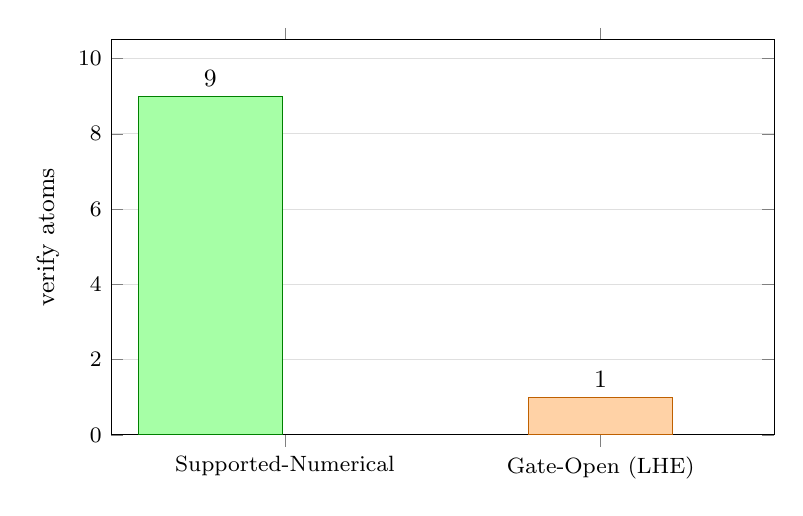
\begin{tikzpicture}
\begin{axis}[
  width=10cm, height=6.6cm,
  ybar,
  bar width=52pt,
  ymin=0, ymax=10.5,
  ylabel={verify atoms},
  symbolic x coords={Numerical, GateOpen},
  xtick={Numerical, GateOpen},
  xticklabels={Supported-Numerical, Gate-Open (LHE)},
  x tick label style={font=\footnotesize},
  tick label style={font=\footnotesize},
  label style={font=\small},
  nodes near coords,
  nodes near coords style={font=\small},
  ymajorgrids,
  grid style={gray!25},
  enlarge x limits=0.55,
]
\addplot[draw=green!50!black,fill=green!35] coordinates {(Numerical,9)};
\addplot[draw=orange!75!black,fill=orange!35,bar shift=0pt] coordinates {(GateOpen,1)};
\end{axis}
\end{tikzpicture}
\end{document}
